% !TEX root = ../TensorOT.tex



\section{Applications}
\label{sec:appli}

This section showcases four different applications of Q-OT to register and interpolate tensor fields.
%
Unless otherwise stated, the data is normalized to the unit cube $[0,1]^d$ (here $d=2$ for images) and discretized on grids of $|I|=|J|=50^d$ points. 
%
The regularization parameter is set to $\epsilon=0.08^2$, the fidelity penalty to $\rho=1$, and the relaxation parameter for Sinkhorn to $\tau_k=\tfrac{1.8 \epsilon}{\epsilon+\rho_k}$. 

% !TEX root = ../TensorOT.tex

%%%%%%%%%%%%%%%%%%%%%%%%%%%%%%%%%%%%%%%%%%%%%%%%%%%%%%%%%
\subsection{Anisotropic Space-varying Procedural Noise}



%%% FIG %%%
\newcommand{\BumpFig}[1]{\includegraphics[width=.17\linewidth,trim=140 10 125 0,clip]{mesh-bump/anisodiffus-#1}}
\newcommand{\TextureImg}[2]{\includegraphics[width=.19\linewidth]{textures/#1/interpol-#2}}
\begin{figure}\centering
\begin{tabular}{@{}c@{\hspace{.5mm}}c@{\hspace{.5mm}}c@{\hspace{.5mm}}c@{\hspace{.5mm}}c@{\hspace{.5mm}}c@{}}
\TextureImg{2d-bump-donut}{render-1}&
\TextureImg{2d-bump-donut}{render-3}&
\TextureImg{2d-bump-donut}{render-5}&
\TextureImg{2d-bump-donut}{render-7}&
\TextureImg{2d-bump-donut}{render-9}&

\includegraphics[height=.19\linewidth]{textures/2d-bump-donut/colorbar.png} \\
\BumpFig{1}&
\BumpFig{3}&
\BumpFig{5}&
\BumpFig{7}&
\BumpFig{9}&\\
$t=0$ & $t=1/4$ & $t=1/2$ & $t=3/4$ & $t=1$
\end{tabular}
\caption{Example of interpolation between two input procedural anisotropic noise function. The PSD tensor field parameterizing the texture are displayed on Figure~\ref{fig:intro}. The colormap used to render the anisotropic texture is displayed on the last column.  
} \label{fig:texture}
\end{figure}
%%% FIG %%%

Texture synthesis using procedural noise functions is widely used in rendering pipelines and video games because of both its low storage cost and the fact that it is typically parameterized by a few meaningful parameters~\cite{LagaeSurvey}. 
%
Following~\cite{LagaImproving} we consider here a spatially-varying Gabor noise function (i.e. a non-stationary Gaussian noise), whose covariance function is parameterized using a PSD-valued field $\mu$. 
%
Quantum optimal transport allows to interpolate and navigate between these noise functions by transporting the corresponding tensor fields. 
%
The initial Gabor noise method makes use of sparse Gabor splattering~\cite{LagaeSurvey} (which enables synthesis at arbitrary resolution and zooming). For simplicity, we rather consider here a more straightfoward method, where the texture $f_{t_0}$ is obtained by stopping at time $t=t_0$ an ansiotropic diffusion guided by the tensor field $\mu$  of a high frequency noise $\Nn$ (numerically a white noise on a grid)
\eq{
	\frac{\partial_t f_t}{\partial t} = \text{div}( \mu \nabla f_t ), \qwhereq
	f_{t=0} \sim \Nn, 
}
where $(\mu \nabla f_t)(x) \eqdef \mu(x) (\nabla f_t(x))$ is the vector field obtained by applying the tensor $\mu(x) \in \Ss_2^+$ to the gradient vector $\nabla f_t(x) \in \RR^2$. 
%
Locally around $x$, the texture is stretched in the direction of the main eigenvector of $\mu(x)$,  highly anisotropic tensor giving rise to elongated ``stripes'' as opposed to isotropic tensor generating ``spots''. 

Numerically, $f$ is discretized on a 2-D grid, and $\mu$ is represented on this grid as a sum of Dirac masses~\eqref{eq-input-measures}. On Euclidian domains $X$, $\nabla$ and div are computed using usual finite difference, while on triangulated mesh, they are implemented using standard piecewise linear finite element primitives. 
%
Figure~\ref{fig:texture} shows two illustrations of this method. Top row generates an animated color texture by indexing a non-linear black-red colormap (displayed on the right) using $f_t$. Bottom row generates an animated bump-mapped surface using $f_t$ to offset the mesh surface in the normal direction. 



% !TEX root = ../TensorOT.tex


%%%%%%%%%%%%%%%%%%%%%%%%%%%%%%%%%%%%%%%%%%%%%%%%%%%%%%%%%
\subsection{Anisotropic Meshing}

Approximation with anisotropic piecewise linear finite elements on a triangulated mesh is a fundamental tool to address tasks such as discretizing partial differential equations, performing surface remeshing~\cite{alliez2003anisotropic} or for image compression~\cite{demaret2006image}.
%
A common practice is to generate triangulation complying with a PSD tensor field $\mu$, i.e. such that a triangle centred at $x$ should be inscribed in the ellipsoid $\enscond{u}{(u-x)^\top \mu(x) (u-x) \leq \de }$ for some $\de$ controlling the triangulation density. 
%
A well known result is that optimal triangle shapes to locally approximate a smooth convex $C^2$ function $f$ is dictated by the Hessian $H f$ of the function~\cite{shewchuk2002good}, so that in practice people use $\mu(x) = |H f(x)|^\al$ for some exponent $\al > 0$ (which is related to the quality measure of the approximation).
%
Figure~\eqref{fig:meshing} shows that Q-OT can be used (using formula~\eqref{eq-interpolating}) to interpolate between two sizing fields $(\mu,\nu)$, which are computed from the Hessian of two initial input images $(f_0,f_1)$.
%
The resulting anisotropic triangulations are defined as geodesic Delaunay triangulation for the Riemannian metric defined by the tensor field, and computed using the method detailed in~\cite{peyre-iccv-09}
%
This interpolation could typically used to track the evolution of the solution of some PDE. 



%%% FIG %%%
\newcommand{\MeshingImg}[2]{\includegraphics[width=.195\linewidth]{meshing/#1/input-#2}}
\begin{figure}\centering
\begin{tabular}{@{}c@{}c@{}c@{}c@{}c@{}}
\MeshingImg{2d-bump-donut}{mesh-1}&
\MeshingImg{2d-bump-donut}{mesh-3}&
\MeshingImg{2d-bump-donut}{mesh-5}&
\MeshingImg{2d-bump-donut}{mesh-7}&
\MeshingImg{2d-bump-donut}{mesh-9}\\
\MeshingImg{images}{mesh-1}&
\MeshingImg{images}{mesh-3}&
\MeshingImg{images}{mesh-5}&
\MeshingImg{images}{mesh-7}&
\MeshingImg{images}{mesh-9}\\
$t=0$ & $t=1/4$ & $t=1/2$ & $t=3/4$ & $t=1$
\end{tabular}
\begin{tabular}{@{}c@{\hspace{1mm}}c@{\hspace{8mm}}c@{\hspace{1mm}}c@{}}
\MeshingImg{images}{images-1}&
\MeshingImg{images}{mesh-1-img}&
\MeshingImg{images}{images-2}&
\MeshingImg{images}{mesh-9-img} \\
$f_0$ \& $\mu$ & & $f_1$ \& $\nu$ &
\end{tabular}
\caption{Two examples of interpolation between two input sizing fields $(\mu_{t=0},\mu_{t=1})=(\mu,\nu)$. 
\textbf{First row:} the sizing fields are displayed on Figure~\ref{fig:intro}.
\textbf{Second row:} the input sizing fields $(\mu_{t=0},\mu_{t=1})=(\mu,\nu)$ are displayed on the last row, and are defined using the absolute valued of the Hessian of the underlying images $(f_0,f_1)$.
} \label{fig:meshing}
\end{figure}
%%% FIG %%%



% !TEX root = ../TensorOT.tex




%%%%%%%%%%%%%%%%%%%%%%%%%%%%%%%%%%%%%%%%%%%%%%%%%%%%%%%%%
\subsection{Diffusion Tensor Imaging}

Diffusion tensor magnetic resonance imaging (DTI) is a popular technique to image the white matter of the brain (see~\cite{wandell2016clarifying} for a recent overview). DTI measures the diffusion of water molecules, which can be compactly encoded using a PSD tensor field $\mu(x) \in \Ss_+^3$, whose anisotropy and size matches the local diffusivity. 
%
A typical goal of this imaging technique is to map the brain anatomical connectivity, and in particular track the  white matter fibers. This requires a careful handling of the tensor's energy (its trace) and anisotropy, so using Q-OT is a perfect fit for such data.

Figure~\ref{fig:dti} shows an application of Q-OT for the interpolation (using~\ref{eq-interpolating}) between 2-D slices from DTI tensor fields $(\mu,\nu)$ acquired on two different subjects. This data is extracted from the studies~\cite{pestilli2014evaluation,takemura2016ensemble}. These two patients exhibit different anatomical connectivity geometries, and Q-OT is able to track the variation in both orientation and magnitude of the diffusion tensors. This figure also compares the different data fidelity parameters $\rho \in \{0.05,1\}$. Selecting $\rho=1$ enforces an overly-strong conservation constraint and leads to interpolation artifacts (in particular some structure are split during the interpolation). In contrast, selecting $\rho=0.05$ introduces enough mass creation/destruction during the interpolation to be able to cope with strong inter-subject variability.

%%% FIG %%%
\newcommand{\DTIimg}[1]{\includegraphics[width=.195\linewidth,trim=85 20 85 20,clip]{dti/#1}}

\begin{figure}\centering
\HighResFig{
\begin{tabular}{@{}c@{\hspace{1mm}}c@{\hspace{1mm}}c@{\hspace{1mm}}c@{\hspace{1mm}}c@{}}
\DTIimg{one-two/interpol-rho1-1}&
\DTIimg{one-two/interpol-rho1-3}&
\DTIimg{one-two/interpol-rho1-5}&
\DTIimg{one-two/interpol-rho1-7}&
\DTIimg{one-two/interpol-rho1-9}\\
\DTIimg{one-two/interpol-rho005-1}&
\DTIimg{one-two/interpol-rho005-3}&
\DTIimg{one-two/interpol-rho005-5}&
\DTIimg{one-two/interpol-rho005-7}&
\DTIimg{one-two/interpol-rho005-9}\\
\DTIimg{four-two/interpol-rho005-1}&
\DTIimg{four-two/interpol-rho005-3}&
\DTIimg{four-two/interpol-rho005-5}&
\DTIimg{four-two/interpol-rho005-7}&
\DTIimg{four-two/interpol-rho005-9}\\
$t=0$ & $t=1/4$ & $t=1/2$ & $t=3/4$ & $t=1$
\end{tabular}
\begin{tabular}{@{}c@{\hspace{2mm}}c@{\hspace{2mm}}c@{}}
\includegraphics[width=.3\linewidth]{dti/one-two/original-trace-1-roi}&
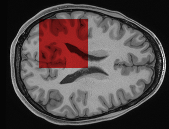
\includegraphics[width=.3\linewidth]{dti/one-two/original-trace-2-roi}&
\includegraphics[width=.3\linewidth]{dti/four-two/original-trace-1-roi}\\
Subject $A$ & Subject $B$ & Subject $C$  
\end{tabular}
}{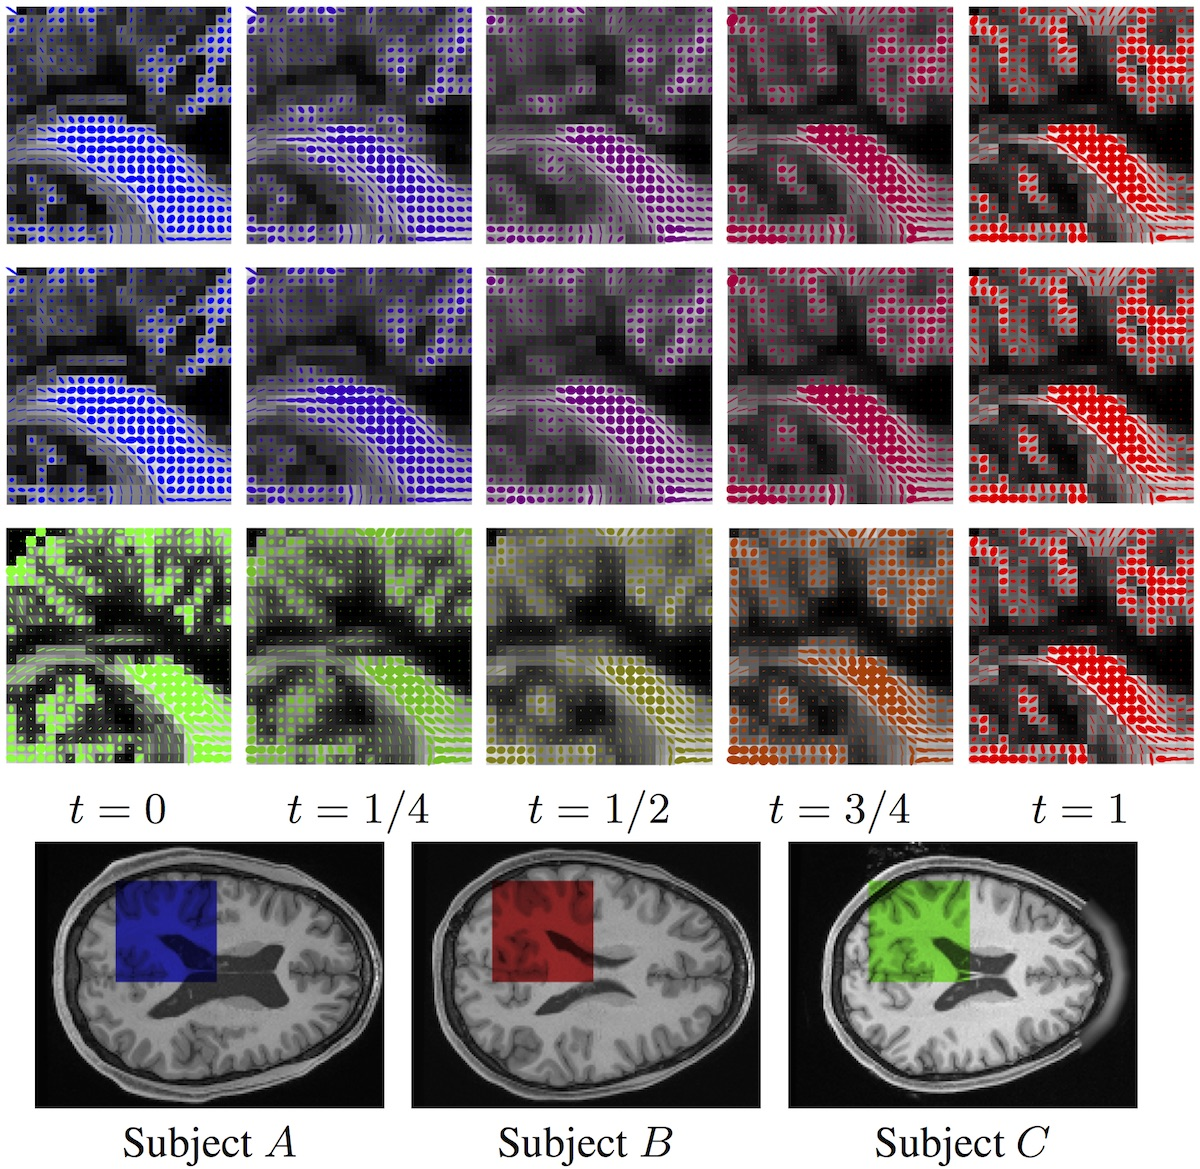
\includegraphics[width=\linewidth]{dti-all}}
\caption{Interpolation between two 2-D slices of 3-D DTI tensor fields $(\mu,\nu)=(\mu_{t=0},\mu_{t=1})$. For readability, only the X/Y components of the tensors are displayed. 
\textbf{First row:} interpolation between subjects $(A,B)$ obtained using $\rho=1$. 
\textbf{Second row:} interpolation between subjects $(A,B)$ obtained using $\rho=0.05$. 
\textbf{Third row:} interpolation between subjects $(C,B)$ obtained using $\rho=0.05$. 
\textbf{Fourth row:} anatomical MRI images of subjects $(A,B,C)$ indicating the region of interest where the computations are performed. 
} \label{fig:dti}
\end{figure}
%%% FIG %%%
% !TEX root = ../TensorOT.tex


%%%%%%%%%%%%%%%%%%%%%%%%%%%%%%%%%%%%%%%%%%%%%%%%%%%%%%%%%
\subsection{Spectral Color Texture Synthesis}

As advocated initially in~\cite{galerne2011random}, a specific class of textured images (so-called micro-textures) is well-modeled using stationary Gaussian fields. In the following, we denote $p$ the pixel positions and $x$ the Fourier frequency indices. For color images, these fields are fully characterized by their mean $m \in \RR^3$ and their Fourier power spectrum, which is a tensor valued field $\mu(x)$ where, for each frequency $x$ (defined on a 2-D grid) $\mu(x) \in \CC^{3 \times 3}$ is a complex positive semi-definite hermitian matrix. 

In practice, $\mu(x)$ is estimated from an exemplar color image $f(p) \in \RR^3$ using an empirical spectrogram 
\eql{\label{eq-power-spectrum}
	\mu(x) \eqdef \frac{1}{K} \sum_{k=1}^K \hat f_k(x) \hat f_k(x)^* \in \CC^{3 \times 3}
}
where $\hat f_k$ is the Fourier transform of $f_k(p) \eqdef f(p) w_k(p)$ (computed using the FFT), $w_k$ are windowing functions centred around $K$ locations in the image plane, and $v^* \in \CC^{1 \times 3}$ denoted the transpose-conjugate of a vector $v \in \CC^{3 \times 1}$. 
%
Increasing the number $K$ of windowed estimations helps to avoid having rank-deficient covariances ($K=1$ leads to a field $\mu$ of rank-1 tensors).

Randomized new textures are then created by generating random samples $F(p) \in \RR^3$ from the Gaussian field, which is achieved by defining the Fourier transform $\hat F(x) \eqdef m + \hat N(x) \sqrt{\mu(x)} \ones_3$, where $N(p)$ is the realization of a Gaussian white noise, and $\sqrt{\cdot}$ is the matrix square root (see~\cite{galerne2011random} for more details).

Figure~\ref{fig:texsynth} shows an application where two input power spectra $(\mu,\nu)$ (computed using~\eqref{eq-power-spectrum} from two input textures exemplars $(f,g)$)  are interpolated using~\eqref{eq-interpolating}, and for each interpolation parameter $t \in [0,1]$ a new texture $F$ is synthesized and displayed.
%
Note that while the Q-Sinkhorn Algorithm~\ref{alg:sinkhorn} is provided for real PSD matrices, it extends verbatim to complex positive hermitian matrices (the matrix logarithm and exponential being defined the same way as for real matrices).

% !TEX root = ../TensorOT.tex


%%% FIG %%%
\newcommand{\TexSynthImg}[1]{\includegraphics[width=.195\linewidth]{texsynth/#1}}
\begin{figure}\centering
\begin{tabular}{@{}c@{\hspace{1mm}}c@{\hspace{1mm}}c@{\hspace{1mm}}c@{\hspace{1mm}}c@{}}
\TexSynthImg{synth1/spectrum-1}&
\TexSynthImg{synth1/spectrum-3}&
\TexSynthImg{synth1/spectrum-5}&
\TexSynthImg{synth1/spectrum-7}&
\TexSynthImg{synth1/spectrum-9}\\
\TexSynthImg{synth1/synthesis-1}&
\TexSynthImg{synth1/synthesis-3}&
\TexSynthImg{synth1/synthesis-5}&
\TexSynthImg{synth1/synthesis-7}&
\TexSynthImg{synth1/synthesis-9}\\
\TexSynthImg{synth2/spectrum-1}&
\TexSynthImg{synth2/spectrum-3}&
\TexSynthImg{synth2/spectrum-5}&
\TexSynthImg{synth2/spectrum-7}&
\TexSynthImg{synth2/spectrum-9}\\
\TexSynthImg{synth2/synthesis-1}&
\TexSynthImg{synth2/synthesis-3}&
\TexSynthImg{synth2/synthesis-5}&
\TexSynthImg{synth2/synthesis-7}&
\TexSynthImg{synth2/synthesis-9}\\
$t=0$ & $t=1/4$ & $t=1/2$ & $t=3/4$ & $t=1$
\end{tabular}
\begin{tabular}{@{}c@{\hspace{1mm}}c@{\hspace{5mm}}c@{\hspace{1mm}}c@{}}
\TexSynthImg{synth1/original-1}&
\TexSynthImg{synth1/original-2}&
\TexSynthImg{synth2/original-1}&
\TexSynthImg{synth2/original-2}\\
$f$  & $g$ & $f$  & $g$ 
\end{tabular}
\caption{\textbf{Row 1 and 3:}  display $\tr(\mu_t(x))$ where $\mu_t$ are the interpolated power spectra. 
\textbf{Rows 2 and 4:} realizations of the Gaussian field parameterized by the power spectra  $\mu_t$. 
\textbf{Row 5:} input texture exemplars from which $(\mu_{t=0},\mu_{t=1})=(\mu,\nu)$ are computed.
} \label{fig:texsynth}
\end{figure}
%%% FIG %%%



